\documentclass[14pt]{beamer}
\usepackage{./Estilos/BeamerUVM}
\usepackage{./Estilos/ColoresLatex}
%Sección para el tema de beamer, con el theme, usercolortheme y sección de footers
\usetheme{Berlin}
\usecolortheme{beaver}
%\useoutertheme{default}
\setbeamercovered{invisible}
% or whatever (possibly just delete it)
\setbeamertemplate{section in toc}[sections numbered]
\setbeamertemplate{subsection in toc}[subsections numbered]
\setbeamertemplate{subsection in toc}{\leavevmode\leftskip=3.2em\rlap{\hskip-2em\inserttocsectionnumber.\inserttocsubsectionnumber}\inserttocsubsection\par}
% \setbeamercolor{section in toc}{fg=blue}
% \setbeamercolor{subsection in toc}{fg=blue}
% \setbeamercolor{frametitle}{fg=blue}
% \setbeamertemplate{caption}[numbered]

\setbeamertemplate{footline}
\beamertemplatenavigationsymbolsempty
\setbeamertemplate{headline}{}


\makeatletter
% \setbeamercolor{section in foot}{bg=gray!30, fg=black!90!orange}
% \setbeamercolor{subsection in foot}{bg=blue!30!yellow, fg=red}
% \setbeamercolor{date in foot}{bg=black, fg=white}
\setbeamertemplate{footline}
{
  \leavevmode%
  \hbox{%
  \begin{beamercolorbox}[wd=.333333\paperwidth,ht=2.25ex,dp=1ex,center]{section in foot}%
    \usebeamerfont{section in foot} \insertsection
  \end{beamercolorbox}%
  \begin{beamercolorbox}[wd=.333333\paperwidth,ht=2.25ex,dp=1ex,center]{subsection in foot}%
    \usebeamerfont{subsection in foot}  \insertsubsection
  \end{beamercolorbox}%
  \begin{beamercolorbox}[wd=.333333\paperwidth,ht=2.25ex,dp=1ex,right]{date in head/foot}%
    \usebeamerfont{date in head/foot} \insertshortdate{} \hspace*{2em}
    \insertframenumber{} / \inserttotalframenumber \hspace*{2ex} 
  \end{beamercolorbox}}%
  \vskip0pt%
}

% \usefonttheme{serif}
\usepackage[clock]{ifsym}
\usepackage{pstricks-add}
\DeclareSIUnit\erg{erg}
\DeclareSIUnit[number-unit-product = {\,}]\cal{cal}

\sisetup{per-mode=symbol}
\resetcounteronoverlays{saveenumi}

% Macro para agregar el logo de UVM en cada slide de la presentación

\addtobeamertemplate{frametitle}{}{%
\begin{tikzpicture}[remember picture,overlay]
\coordinate (logo) at ([xshift=-1.5cm,yshift=-0.8cm]current page.north east);
% \fill[devryblue] (logo) circle (.9cm);
% \clip (logo) circle (.75cm);
\node at (logo) {
\includegraphics[width=2.1cm]{Imagenes/logo_UVM.png}};
\end{tikzpicture}}


\title{\Large{Movimiento circular} \\ \normalsize{Física III}}
\date{}

\begin{document}
\maketitle

\section*{Contenido}
\frame[allowframebreaks]{\frametitle{Contenido} \tableofcontents[currentsection, hideallsubsections]}

\section{Movimiento circular}
\frame{\tableofcontents[currentsection, hideothersubsections]}
\subsection{Definición}

\begin{frame}
\frametitle{El movimiento circular}
Un objeto describe un \textocolor{ao}{movimiento circular} cuando su trayectoria es una circunferencia.
\end{frame}
\begin{frame}
\frametitle{El movimiento circular}
En este movimiento el vector \textocolor{burgundy}{velocidad varía constantemente} de dirección, \pause y su \textocolor{coolblack}{magnitud puede variar} o permanecer constante.
\end{frame}
\begin{frame}
\frametitle{El movimiento circular}
Por tanto, en un movimiento circular un cuerpo se puede mover con rapidez constante o no, \pause pero su \textocolor{red}{aceleración formará siempre un ángulo recto} (\ang{90}) con su velocidad \pause y se desplazará formando un círculo.
\end{frame}
\begin{frame}
\frametitle{La aceleración circular}
La aceleración que recibe el cuerpo \textocolor{coquelicot}{está dirigida hacia el centro del círculo} y recibe el nombre de \textocolor{bulgarianrose}{aceleración normal}, \pause \textocolor{bulgarianrose}{radial} \pause o \textocolor{bulgarianrose}{centrípeta}.
\end{frame}

\subsection{Conceptos}

\begin{frame}
\frametitle{Ángulo}
Es la abertura comprendida entre dos radios cualesquiera, que limitan un arco de circunferencia.
\end{frame}
\begin{frame}
\frametitle{Radián}
Es el ángulo central al que corresponde un arco de longitud igual al radio.
\end{frame}
\begin{frame}
\frametitle{Vector de posición}
Si observamos el movimiento de un objeto colocado encima de un disco que gira, \pause podemos precisar su posición si tomamos como origen del sistema de referencia al centro de la trayectoria circular.
\end{frame}
\begin{frame}
\frametitle{Vector de posición}
De esta forma, el vector que nos indicará su posición para cada intervalo de tiempo se encontrará determinado por el radio de la circunferencia, mismo que permanece constante.
\end{frame}
\begin{frame}
\frametitle{Vector de posición}
Por tanto, el vector de posición tendrá una magnitud constante y su dirección será la misma que tenga el radio de la circunferencia.
\end{frame}
\begin{frame}
\frametitle{Vector de posición}
Cuando el objeto colocado sobre el disco se desplace, su cambio de posición se podrá expresar mediante desplazamientos del vector de posición, lo cual dará lugar a desplazamientos angulares.
\end{frame}
\begin{frame}
\frametitle{Desplazamiento angular}
Por tanto, el desplazamiento angular es la magnitud física que cuantifica la magnitud de la rotación que experimenta un objeto de acuerdo con su ángulo de giro.
\end{frame}
\begin{frame}
\frametitle{Desplazamiento angular}
El desplazamiento angular se representa por la letra griega $\theta$ (theta), \pause sus unidades de medida son: 
\pause
\setbeamercolor{item projected}{bg=pansypurple,fg=white}
\setbeamertemplate{enumerate items}{%
\usebeamercolor[bg]{item projected}%
\raisebox{1.5pt}{\colorbox{bg}{\color{fg}\footnotesize\insertenumlabel}}%
}
\begin{enumerate}[<+->]
\item El radián cuando el sistema usado es el internacional.
\item En grados sexagesimales.
\item Revoluciones.
\end{enumerate}
\end{frame}
\begin{frame}
\frametitle{Desplazamiento angular}
\vspace*{-1cm}
\begin{figure}
    \centering
    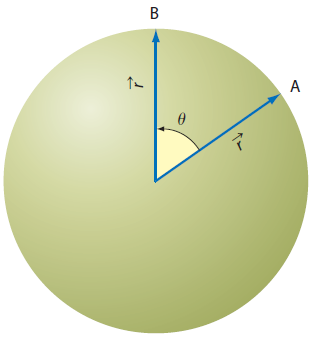
\includegraphics[scale=0.75]{Imagenes/Movimiento_Circular_01.png}
\end{figure}
\end{frame}
\begin{frame}
\frametitle{Desplazamientos angulares}
\vspace*{-1cm}
\begin{figure}
    \centering
    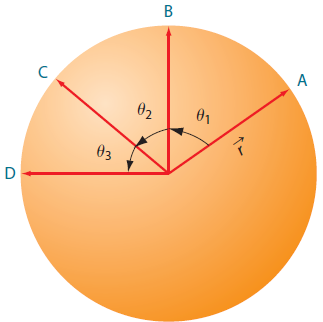
\includegraphics[scale=0.75]{Imagenes/Movimiento_Circular_02.png}
\end{figure}
\end{frame}

\subsection{Conceptos necesarios}

\begin{frame}
\frametitle{El periodo}
Es el tiempo que tarda un objeto en dar una vuelta completa o en completar un ciclo.
\end{frame}
\begin{frame}
\frametitle{El periodo}
En el sistema internacional, la unidad del periodo es el segundo.
\pause
\begin{align*}
T = \dfrac{\text{segundos transcurridos}}{\text{1 ciclo}}
\end{align*}
\end{frame}
\begin{frame}
\frametitle{La frecuencia}
Es el número de vueltas, revoluciones o ciclos que efectúa un móvil en un segundo.
\pause
\begin{align*}
f = \dfrac{\text{número de ciclos}}{\text{1 segundo}}
\end{align*}
Las unidades de la frecuencia es el Hertz (\si{\hertz}).
\end{frame}

\section{Dinámica circular}
\frame{\tableofcontents[currentsection, hideothersubsections]}
\subsection{Velocidad}

\begin{frame}
\frametitle{Velocidad angular}
La magnitud de la velocidad angular representa el cociente entre la magnitud del desplazamiento angular de un objeto y el tiempo que tarda en efectuarlo:
\pause
\begin{align*}
\omega = \dfrac{\theta}{t} \hspace{1cm} \left[ \dfrac{\text{rad}}{\unit{\second}} \right]
\end{align*}
\end{frame}
\begin{frame}
\frametitle{Velocidad angular}
\vspace*{-1cm}
\begin{align*}
\omega = \dfrac{\theta}{t} \hspace{1cm} \left[ \dfrac{\text{rad}}{\unit{\second}} \right]
\end{align*}    
donde:
\setbeamercolor{item projected}{bg=pastelgreen,fg=black}
\setbeamertemplate{enumerate items}{%
\usebeamercolor[bg]{item projected}%
\raisebox{1.5pt}{\colorbox{bg}{\color{fg}\footnotesize\insertenumlabel}}%
}
\begin{enumerate}[<+->]
\item $\omega$ es la magnitud de la velocidad angular.
\item $\theta$ es la magnitud del desplazamiento angular.
\item $t$ es el tiempo en que se efectúa el desplazamiento.
\end{enumerate}
\end{frame}
\begin{frame}
\frametitle{La velocidad angular}
La magnitud de la velocidad angular se puede expresar en \textocolor{patriarch}{función de los cambios} en su desplazamiento angular con respecto al cambio en el tiempo, de la siguiente forma:
\pause
\begin{eqnarray*}
\begin{aligned}
\omega = \dfrac{\Delta \theta}{\Delta t} = \pause \dfrac{\theta_{2} - \theta_{1}}{t_{2} - t_{1}}
\end{aligned}
\end{eqnarray*}
\end{frame}
\begin{frame}
\frametitle{La velocidad angular}
La magnitud de la velocidad angular también se puede determinar si se conoce su periodo $(T)$ es decir, el tiempo que tarda en dar una vuelta completa o una revolución:
\pause
\begin{align*}
\ang{360}  = 2 \, \pi \, \text{radianes}
\end{align*}
\end{frame}
\begin{frame}
\frametitle{La velocidad angular}
La expresión que se utiliza es:
\pause
\begin{eqnarray*}
\begin{aligned}
\omega = \dfrac{2 \, \pi \, \text{rad}}{T} = \pause \dfrac{2 \, \pi}{T} \hspace{1cm} \left[ \dfrac{\text{rad}}{\unit{\second}} \right]
\end{aligned}
\end{eqnarray*}
\end{frame}
\begin{frame}
\frametitle{La velocidad angular}
Pero como $T = 1 / f$, la velocidad angular se determina también por:
\pause
\begin{align*}
\omega = 2 \, \pi \, f \hspace{1cm} \left[ \dfrac{\text{rad}}{\unit{\second}} \right]
\end{align*}
\end{frame}

\subsection{Velocidad angular media}

\begin{frame}
\frametitle{La velocidad angular media}
Cuando la velocidad angular de un objeto \textocolor{red}{no es constante o uniforme}, \pause podemos determinar la magnitud de la velocidad angular media al conocer las magnitudes de la velocidad angular inicial y su velocidad angular final:
\pause
\begin{align*}
\omega_{m} = \dfrac{\omega_{f} + \omega_{i}}{2}
\end{align*}
\end{frame}
\begin{frame}
\frametitle{La velocidad angular media}
\vspace*{-1cm}
\begin{align*}
\omega_{m} = \dfrac{\omega_{f} + \omega_{i}}{2}
\end{align*}
Donde:
\setbeamercolor{item projected}{bg=persianindigo,fg=white}
\setbeamertemplate{enumerate items}{%
\usebeamercolor[bg]{item projected}%
\raisebox{1.5pt}{\colorbox{bg}{\color{fg}\footnotesize\insertenumlabel}}%
}
\begin{enumerate}[<+->]
\item $\omega_{m}$ es la magnitud de la vel. angular.
\item $\omega_{f}$ es la magnitud de la vel. angular final.
\item $\omega_{0}$ es la magnitud de la vel. angular inicial.
\end{enumerate}
\end{frame}

\subsection{Velocidad lineal o tangencial}

\begin{frame}
\frametitle{Velocidad lineal}
Cuando un objeto se encuentra girando, \pause cada una de las partículas del mismo se mueve a lo largo de la circunferencia descrita por él con una velocidad lineal cuya magnitud será mayor, \pause  a medida que aumenta el radio de la circunferencia.
\end{frame}
\begin{frame}
\frametitle{Velocidad tangencial}
Esta velocidad lineal también recibe el nombre de \textocolor{red-violet}{velocidad tangencial}, \pause porque la dirección de la velocidad siempre es tangente a la circunferencia recorrida por la partícula.
\end{frame}
\begin{frame}
\frametitle{Velocidad tangencial}
Representa la magnitud de la velocidad que llevaría ésta si saliera disparada tangencialmente.
\end{frame}
\begin{frame}
\frametitle{Velocidad tangencial}
\vspace*{-1cm}
\begin{figure}
    \centering
    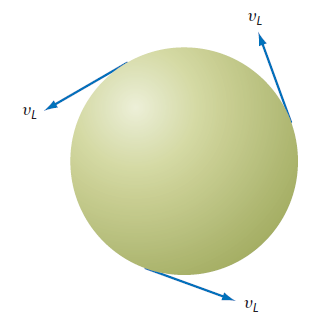
\includegraphics[scale=0.75]{Imagenes/Movimiento_Circular_03.png}
\end{figure}
\end{frame}
\begin{frame}
\frametitle{Magnitud velocidad tangencial}
Para \textocolor{red(ryb)}{calcular la magnitud} de la velocidad tangencial o lineal se usa la ecuación:
\pause
\begin{align*}
v_{L} = \dfrac{2 \, \pi \, r}{T}
\end{align*}
\end{frame}
\begin{frame}
\frametitle{Magnitud velocidad tangencial}
\begin{align*}
v_{L} = \dfrac{2 \, \pi \, r}{T}
\end{align*}
donde:
\pause
\setbeamercolor{item projected}{bg=rose,fg=white}
\setbeamertemplate{enumerate items}{%
\usebeamercolor[bg]{item projected}%
\raisebox{1.5pt}{\colorbox{bg}{\color{fg}\footnotesize\insertenumlabel}}%
}
\begin{enumerate}[<+->]
\item $r$ es el radio de la circunferencia en metros.
\item $T$ es el periodo en segundos.
\item $v_{L}$ es la velocidad lineal en \unit{\meter\per\second}
\end{enumerate}
\end{frame}
\begin{frame}
\frametitle{Magnitud velocidad tangencial}

Como la velocidad angular es $\omega = 2 \, \pi /T$, la magnitud de la velocidad lineal se expresa también como:
\pause
\begin{align*}
v_{L} = \omega \cdot r
\end{align*}
\end{frame}
\begin{frame}
\frametitle{Ejercicio 1}
¿Cuál es la magnitud de la velocidad angular de una llanta de un camión que gira desplazándose \SI{12}{\radian} en \SI{0.5}{\second}?
\end{frame}
\begin{frame}
\frametitle{Ejercicio 2}
Determina la magnitud de la velocidad angular y la
frecuencia de una pelota atada a un hilo, si gira con un periodo de \SI{0.6}{\second}.
\end{frame}
\begin{frame}
\frametitle{Ejercicio 3}
Halla la magnitud de la velocidad angular y el periodo de una rueda que gira con una frecuencia de \num{430} revoluciones por minuto.
\end{frame}
\begin{frame}
\frametitle{Ejercicio 4}
Calcular la magnitud de la velocidad lineal de una partícula cuyo radio de giro es de \SI{25}{\centi\meter} y tiene un periodo de \SI{0.01}{\second}.
\end{frame}

\section{MCUA}
\frame{\tableofcontents[currentsection, hideothersubsections]}
\subsection{Aceleración angular}

\begin{frame}
\frametitle{El MCUA}
El \textocolor{rossocorsa}{movimiento circular uniformemente acelerado} \pause se presenta cuando un móvil con trayectoria circular \textocolor{ao}{aumenta} o \textocolor{red}{disminuye} en cada unidad de tiempo la magnitud de su velocidad angular en forma constante.
\end{frame}
\begin{frame}
\frametitle{El MCUA}
Por lo que la magnitud de su \textocolor{ruddy}{aceleración angular permanece constante}.
\end{frame}

\subsection{Aceleración angular media}

\begin{frame}
\frametitle{Aceleración angular media}
Cuando durante el movimiento circular de un móvil su velocidad angular no permanece constante, \pause sino que varía, decimos que sufre una \textocolor{bole}{aceleración angular}.
\end{frame}
\begin{frame}
\frametitle{Aceleración angular media}
Cuando la velocidad angular varía es conveniente determinar cuál es la magnitud de su aceleración angular media, misma que se expresa de la siguiente manera:
\pause
\begin{align*}
\alpha = \dfrac{\omega_{f} - \omega_{i}}{t_{f} - t_{i}} \hspace{1cm} \left[ \unit{\radian\per\square\second} \right]
\end{align*}
\end{frame}

\subsection{Aceleración centrípeta}

\begin{frame}
\frametitle{Aceleración centrípeta}
La \textocolor{cobalt}{aceleración centrípeta} es la aceleración experimentada por un objeto que se mueve en una trayectoria curvilínea, como una circunferencia.
\end{frame}
\begin{frame}
\frametitle{Aceleración centrípeta}
Esta aceleración \textocolor{red}{siempre está dirigida hacia el centro} de la trayectoria circular \pause y es \textocolor{cardinal}{perpendicular a la velocidad tangencial} del objeto en cualquier punto dado de la trayectoria.
\end{frame}
\begin{frame}
\frametitle{Aceleración centrípeta}
\vspace*{-1cm}
\begin{figure}
\begin{tikzpicture}
    \draw (0, 0) circle (2cm);
    \draw [-stealth, thick] (2, 0) -- (0.5, 0) node [midway, above] {$a_{c}$}; 
    \draw [-stealth, thick] (2, 0) -- (2, 2.5) node [midway, right] {$v_{T}$}; 
\end{tikzpicture}
\end{figure}
\end{frame}
\begin{frame}
\frametitle{Magnitud de la a. centrípeta}
La magnitud de la aceleración centrípeta $(a_{c})$ se calcula utilizando la siguiente fórmula:
\begin{align*}
a_{c} = \dfrac{v^{2}}{r} \hspace{1cm} \left[ \unit[per-mode=fraction]{\meter\per\square\second} \right]
\end{align*}
\pause
Donde:
\setbeamercolor{item projected}{bg=bananayellow,fg=black}
\setbeamertemplate{enumerate items}{%
\usebeamercolor[bg]{item projected}%
\raisebox{1.5pt}{\colorbox{bg}{\color{fg}\footnotesize\insertenumlabel}}%
}
\begin{enumerate}[<+->]
\item $v$ es la velocidad lineal del objeto.
\item $r$ es el radio de la trayectoria circular.
\end{enumerate}
\end{frame}

\subsection{Ecuaciones MCUA}

\begin{frame}
\frametitle{Las ecuaciones en MCUA}
Las ecuaciones empleadas para el MCUA son las mismas que se utilizan para el MRUA con las siguientes
variantes.
\end{frame}
\begin{frame}
\frametitle{Las ecuaciones en MCUA}
\setbeamercolor{item projected}{bg=rust,fg=black}
\setbeamertemplate{enumerate items}{%
\usebeamercolor[bg]{item projected}%
\raisebox{1.5pt}{\colorbox{bg}{\color{fg}\footnotesize\insertenumlabel}}%
}
\begin{enumerate}[<+->]
\item En lugar de magnitud del desplazamiento en metros hablaremos de magnitud del desplazamiento angular en radianes ($\theta$ en lugar de d).
\seti
\end{enumerate}
\end{frame}
\begin{frame}
\frametitle{Las ecuaciones en MCUA}
\setbeamercolor{item projected}{bg=rust,fg=black}
\setbeamertemplate{enumerate items}{%
\usebeamercolor[bg]{item projected}%
\raisebox{1.5pt}{\colorbox{bg}{\color{fg}\footnotesize\insertenumlabel}}%
}
\begin{enumerate}[<+->]
\conti
\item La magnitud de la velocidad en \unit{\meter\per\second} será sustituida por la magnitud de la velocidad angular en \unit{\radian\per\second} ($\omega$ en lugar de $v$).
\seti
\end{enumerate}
\end{frame}
\begin{frame}
\frametitle{Las ecuaciones en MCUA}
\setbeamercolor{item projected}{bg=rust,fg=black}
\setbeamertemplate{enumerate items}{%
\usebeamercolor[bg]{item projected}%
\raisebox{1.5pt}{\colorbox{bg}{\color{fg}\footnotesize\insertenumlabel}}%
}
\begin{enumerate}[<+->]
\conti
\item La magnitud de la aceleración en \unit{\meter\per\square\second} se cambiará por la magnitud de la aceleración angular en \unit{\radian\per\square\second} ($\alpha$ en lugar de a)
\end{enumerate}
\end{frame}
\begin{frame}
\frametitle{Magnitud de los desplazamientos angulares}
\vspace*{-1cm}
\begin{eqnarray*}
\begin{aligned}
\theta &= \omega_{0} \, t + \dfrac{\alpha \, t^{2}}{2} \\[0.5em] \pause
\theta &= \dfrac{\omega_{f}^{2} - \omega_{0}^{2}}{2 \, \alpha} \\[0.5em] \pause
\theta &= \dfrac{\omega_{f} + \omega_{0}}{2} \, t
\end{aligned}
\end{eqnarray*}
\end{frame}
\begin{frame}
\frametitle{Magnitud de los desplazamientos angulares}
Si el objeto parte del reposo su velocidad angular inicial $(\omega_{0})$ es cero, y las tres ecuaciones anteriores se reducen a:
\end{frame}
\begin{frame}
\frametitle{Magnitud de los desplazamientos angulares}
\vspace*{-1cm}
\begin{eqnarray*}
\begin{aligned}
\theta &= \dfrac{\alpha \, t^{2}}{2} \\[0.5em] \pause
\theta &= \dfrac{\omega_{f}^{2}}{2 \, \alpha} \\[0.5em] \pause
\theta &= \dfrac{\omega_{f}}{2} \, t
\end{aligned}
\end{eqnarray*}
\end{frame}
\begin{frame}
\frametitle{Velocidades angulares finales}
Para calcular la magnitud de las velocidades angulares finales:
\end{frame} 
\begin{frame}
\frametitle{Velocidades angulares finales}
\vspace*{-1cm}
\begin{eqnarray*}
\begin{aligned}
\omega_{f} &= \omega_{0} + \alpha \, t \\[0.5em] \pause
\omega_{f} &= \omega_{0}^{2} + 2 \, \alpha \, \theta
\end{aligned}
\end{eqnarray*}
\end{frame}
\begin{frame}
\frametitle{Velocidades angulares finales}
Si el objeto parte del reposo su velocidad inicial $(\omega_{0})$ es cero, y las dos ecuaciones anteriores se reducen a:
\end{frame}
\begin{frame}
\frametitle{Velocidades angulares finales}
\vspace*{-1cm}
\begin{eqnarray*}
\begin{aligned}
\omega_{f} &= \alpha \, t \\[0.5em] \pause
\omega_{f} &= 2 \, \alpha \, \theta
\end{aligned}
\end{eqnarray*}
\end{frame}
\begin{frame}
\frametitle{Ejercicio 1}
En una pista circular de radio \SI{100}{\meter}, un auto le da dos vueltas en cada minuto.
\end{frame}
\begin{frame}
\frametitle{Ejercicio 1}
\setbeamercolor{item projected}{bg=cobalt,fg=white}
\setbeamertemplate{enumerate items}{%
\usebeamercolor[bg]{item projected}%
\raisebox{1.5pt}{\colorbox{bg}{\color{fg}\footnotesize\insertenumlabel}}%
}
\begin{enumerate}[<+->]
\item ¿Cuál es el periodo del movimiento del auto?
\item ¿Cuál es la distancia que recorre en cada ciclo?
\item ¿Qué valor tiene la velocidad lineal del vehículo?
\item ¿Cuánto vale su aceleración centrípeta?
\item ¿Cuál es su velocidad angular?
\end{enumerate}
\end{frame}
\begin{frame}
\frametitle{Ejercicios en clase}
Los siguientes ejercicios se resolverán en clase y se entregarán en el cuaderno para firma.
\end{frame}
\begin{frame}
\frametitle{Ejercicios en clase}
Se otorgará un punto por cada ejercicio, siempre y cuando esté bien resuelto:
\setbeamercolor{item projected}{bg=black,fg=white}
\setbeamertemplate{enumerate items}{%
\usebeamercolor[bg]{item projected}%
\raisebox{1.5pt}{\colorbox{bg}{\color{fg}\footnotesize\insertenumlabel}}%
}
\begin{enumerate}[<+->]
\item Datos.
\item Expresión(es)
\item Sustitución.
\item Manejo de Unidades.
\end{enumerate}
\end{frame}
\begin{frame}
\frametitle{Ejercicios en clase}
Solo se firmará en la clase del día de hoy.
\end{frame}
\begin{frame}
\frametitle{Ejercicio 2}
Una polea motriz de \SI{6}{\centi\meter} de diámetro se hace girar a 9 rev/s.
\setbeamercolor{item projected}{bg=cobalt,fg=white}
\setbeamertemplate{enumerate items}{%
\usebeamercolor[bg]{item projected}%
\raisebox{1.5pt}{\colorbox{bg}{\color{fg}\footnotesize\insertenumlabel}}%
}
\begin{enumerate}[<+->]
\item ¿Cuál es la aceleración centrípeta en un punto localizado en el borde de la polea?
\item ¿Cuál sería la velocidad lineal de una banda accionada por la polea?
\end{enumerate}
\end{frame}
\begin{frame}
\frametitle{Ejercicio 3}
Un objeto está atado a una cuerda y se mueve en un círculo horizontal de \SI{90}{\centi\meter} de radio. Sin considerar los efectos de la gravedad y supóngamos que el objeto gira con una frecuencia de 80 rpm.
\\
\bigskip
\pause
Determina la velocidad lineal $(v_{T})$ y la aceleración centrípeta $(a_{c})$.
\end{frame}
\begin{frame}
\frametitle{Ejercicio 4}
Un ventilador gira dando $120$ vueltas en \SI{1}{\minute}, si la longitud de cada aspa es de \SI{30}{\centi\meter}, y al apagarse se detiene después de \SI{80}{\second}:
\setbeamercolor{item projected}{bg=cobalt,fg=white}
\setbeamertemplate{enumerate items}{%
\usebeamercolor[bg]{item projected}%
\raisebox{1.5pt}{\colorbox{bg}{\color{fg}\footnotesize\insertenumlabel}}%
}
\begin{enumerate}[<+->]
\item ¿Cuál es su aceleración angular?
\item ¿Cuál es la aceleración centrípeta de un punto a la mitad del aspa?
\end{enumerate}
\end{frame}

\end{document}